% programming model
% ecall and ocall

\subsubsection{Overview of SGX-enabled applications}

Using the recently released Intel SGX SDK~\cite{sgxsdk}, we implmented the \tc
Server as an SGX-enabled application in C++. The programming model employed by
the SDK is that the major body of an SGX-enabled application remains an
ordinary user-space application, while an relatively small piece of security-sensitive code
is teased out and runs in an isolated environment, namely in an SGX enclave.

The enclave part of an SGX-enabled application can be
viewed as a shared library exposing APIs, referred to as \emph{ecalls} by~\cite{sgxsdk},
to be invoked by the untrusted application. However, unlike a share library,  
once ecalls are invoked, the control is transferred to the 
enclave code until it finishes or some special event happens~\cite{sgxmanual}.
As we assume SGX provides a perfect isolation, the untrusted application can not
observe or alter the execution of ecalls.

In addition, the SGX SDK implements a mechanism called \emph{ocall} with which enclave
programs can invoke functions defined outside of the enclave. In essence,
calling an ocall causes the enclave program first to exit the enclave. Once the
ocall is fulfilled, execution is transferred back to the calling enclave. 
Although it is permissible to make arbitrary ocalls, special caution must be 
taken as ocalls are fulfilled in the untrusted world.
The ocall interface between the \encname and the \medname is carefully designed
in the security model of \tc.

\begin{figure}[h]
    \centering
    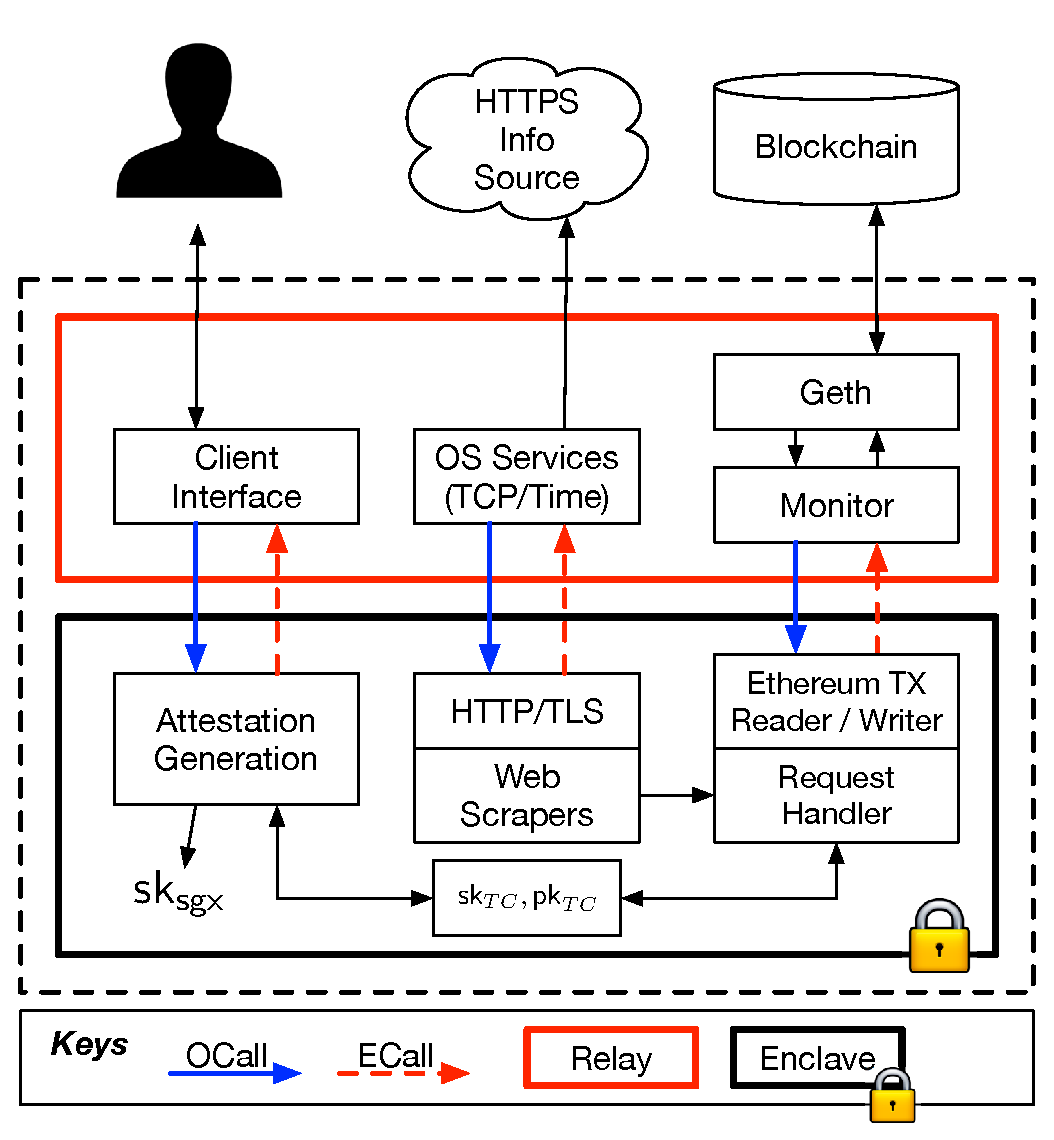
\includegraphics[width=0.45\textwidth]{figures/impl}
    \caption{Components of \tc Server}
    \label{fig:tcserver_impl}
\end{figure}

In the context of TC Server, Fig~\ref{fig:engineprotocol} is implmented as the
enclave part, which encompasses a TLS layer, a (partial) HTTP layer, a set of
algorithms that extract information from web pages, and a request handler that
can parse and generate Ethereum transactions signed with \skTC. The untrusted
part of \tc Server implements Fig~\ref{fig:relayprotocol}, which roughly
encompasses three parts: an access point to various OS services, an interface
with Ethereum blockchain and an interface with clients.
Fig~\ref{fig:tcserver_impl} summarizes these components and their interaction.


\subsubsection{The \medname}

\paragraph{Client Interface.} As described in Section \ref{sec:architecture},
a client starts using \tc by requesting and verifying an attestation.  The
Client Interface part of \medname is dedicated for doing this.  The Client Interface 
listens for requests over network and calls into the Attestation Generation logic in the
enclave (by making an ecall) to get an attestation, along with an Unix timestamp
signed by \pkTC, and forward both to the requesting client. The EPID group
signature can verified by accessing Intel Attestation Service (IAS)~\cite{}. 

\paragraph{OS Services.} The \encname relies on \medname to access networking and 
time services provided by the OS. This is implemented as ocalls.
Since the \encname is potentially malicious, the ocall interface is carefully
designed.

\paragraph{Blockchain Interface.} The \medname is responsible to watch the
blockchain for incoming requests and insert transactions to the blockchain to
deliver datagrams. To interact with the Ethereum blockchain, we incorporated an
official Ethereum client (geth~\cite{geth} in particular) into the \medname.
Geth client can be configured to setup a JSON RPC server through which the
Monitor can communicate with the blockchain indirectly by sending RPC calls to
geth. For example, to insert a signed transaction, the Monitor can simply call
\texttt{eth\_sendRawTransaction} with the bytes array of the serialized
transaction, and geth do the rest of the work. Looping an Ethereum
client into \medname saves us the cost of reinventing the wheel. 
Note that the signing of transactions is done within the enclave, as the key
\pkTC only accessible to the enclave program.

\subsubsection{The \encname}

\paragraph{HTTPS in the \encname.} 
The \encname needs the TLS layer to talk with remote HTTPS web servers.  We
ported a TLS library (mbedTLS) into the SGX environment so it can be used within
the enclave.  To verify the certificates presented by remote servers, a
collection of trusted root CAs are manually selected \xxx[Fan]{what's the best
practice? Maybe we can choose the same root CAs as Chrome or Firefox?} and their
certificates are hardcoded in the enclave program. A certificate is verified
only if it is finally issued by one of the trusted root CA.

\paragraph{Web Scrapers.} Extracting useful information from a given website is
implemented in a ad-hoc manner. For the purpose of demonstration, we implemented
three web scrapers as examples. \xxx[Fan]{Elaborate}.

\paragraph{Request Handler} Request handler has two jobs: 1) to parse the
request which is serialized in the format specified by Ethereum ABI, decrypt it if encrypted under
\pkTC, and dispatch it to the right scraper; 2) to generate a Ethereum
transaction, sign it with \pkTC and serialize it properly so that it can be
inserted to the blockchain. In essence, we implemented the Ethereum ABI and RLP which
specifies the serialization of arguments and transactions respectively.
In addition, the signature algorithm used in signing Ethereum transactions is
ECDSA on the curve Secp256k1. SHA3 is used to generate message digests.

\paragraph{Attestation Generation} \xxx[Fan]{Elaborate.}
